% Chapter Template

\chapter{Results and Analysis} % Main chapter title

\label{c5} % Change X to a consecutive number; for referencing this chapter elsewhere, use \ref{ChapterX}

\section{Results and Analysis}

\pagebreak
% Please add the following required packages to your document preamble:
% \usepackage{longtable}
% Note: It may be necessary to compile the document several times to get a multi-page table to line up properly

\begin{landscape}
\setlength{\tabcolsep}{3pt}
{\renewcommand{\arraystretch}{1}%
\begin{longtable}{|p{0.2\linewidth}|p{0.06\linewidth}|p{0.06\linewidth}|p{0.06\linewidth}|p{0.06\linewidth}|p
        {0.06\linewidth}|p{0.06\linewidth}|p{0.06\linewidth}|p{0.06\linewidth}|p{0.06\linewidth}|}%{|l|r|r|r|r|r|r|r|r|}
    \caption{All Datasets RMSE.}
\label{tab:RMSE_A_d}\\
\hline
\textbf{DataSets} & \textbf{BiLS- TM} & \textbf{CNN} & \textbf{GRU} & \textbf{Seq2- Seq} & \textbf{V-LSTM} & \textbf{S-LSTM} & \textbf{CNN\_ Bi-LSTM} & \textbf{CNN\_ LSTM} & \textbf{GRU\_ Bi-LSTM} \\ \hline
\endfirsthead
%
\endhead
%
\textbf{BHIWADI}        & 23.13 & 57.2  & 22.34 & 24.2  & 19.6  & 48.14 & 45.98 & 43.5  & 35.3  \\ \hline
\textbf{JODHPUR}        & 27.54 & 26.68 & 32.94 & 22.35 & 22.08 & 50    & 40.87 & 43.55 & 52.63 \\ \hline
\textbf{SINGRAULI}      & 10.92 & 15.5  & 27.34 & 21.61 & 13.63 & 17.79 & 50.61 & 22.2  & 26.5  \\ \hline
\textbf{ANKLESHWAR}     & 18.53 & 16.68 & 37.15 & 23.78 & 18.38 & 46.28 & 62.85 & 68.72 & 69.38 \\ \hline
\textbf{LUDHIANA}       & 8.4   & 11.12 & 22.14 & 10.1  & 8.3   & 21.15 & 25.66 & 24.76 & 23.77 \\ \hline
\textbf{DURGAPUR}       & 6.14  & 8.27  & 20.34 & 9.48  & 8.78  & 15.28 & 9.62  & 13.76 & 24.39 \\ \hline
\textbf{YAMUNA\_NAGAR}  & 37.34 & 34.57 & 56.27 & 36.33 & 38.18 & 66.14 & 72.39 & 45.63 & 74.13 \\ \hline
\textbf{CHARKHI\_DADRI} & 18.42 & 20.43 & 27.96 & 18.43 & 18.06 & 40.71 & 46.16 & 45.27 & 43.48 \\ \hline
\textbf{JIND}           & 24.17 & 26.42 & 34.35 & 25.85 & 19.41 & 79.22 & 62.13 & 43.59 & 50.95 \\ \hline
\textbf{KURUKSHETRA}    & 27.14 & 72.03 & 43.56 & 27.32 & 26.7  & 65.77 & 39.71 & 88.12 & 53.74 \\ \hline
\textbf{SONIPAT}        & 12.56 & 15.98 & 22.4  & 15.41 & 10.9  & 43.02 & 24.01 & 22.96 & 46.77 \\ \hline
\textbf{DHARUHERA}      & 26.74 & 28.93 & 34.6  & 24.06 & 25.19 & 53.18 & 31.93 & 35.01 & 46.22 \\ \hline
\textbf{AMBALA}         & 22.58 & 28.96 & 41.08 & 19.92 & 16.92 & 57.43 & 40.71 & 34.14 & 63.85 \\ \hline
\textbf{HISAR}          & 28.34 & 66.79 & 47.93 & 33.98 & 30.99 & 63.29 & 43.16 & 49.1  & 62.46 \\ \hline
\textbf{FATEHABAD}      & 14.37 & 38.36 & 72.71 & 15.51 & 15.58 & 38.38 & 74.38 & 76.75 & 72.64 \\ \hline
\textbf{BULANDSHAHR}    & 7.39  & 8.87  & 19.79 & 11.19 & 7.2   & 14.98 & 9.61  & 13.16 & 11.51 \\ \hline
\textbf{MUZAFFARNAGAR}  & 11.88 & 16.13 & 13.72 & 14.2  & 12.75 & 22.21 & 15.91 & 23.6  & 21.9  \\ \hline

\end{longtable}}
\end{landscape}


\begin{table}[!htp]
\centering
\setlength{\tabcolsep}{3pt}
{\renewcommand{\arraystretch}{1}%
    \caption{Average Rankings of RMSE by (N*N) Friedman Test}
\label{tab:RMSE_Rnk}
\begin{tabular}{|p{0.2\linewidth}|p{0.1\linewidth}|}
\hline
Algorithm&Ranking\\\hline
BiLSTM & 2.1176\\ \hline
CNN & 4.2941\\\hline
GRU & 5.7059\\\hline
Seq2Seq & 3.1176\\\hline
V-LSTM & 1.7059\\\hline
S-LSTM & 7.1176\\\hline
CNN-BiLSTM & 6.5294\\\hline
CNN-LSTM & 6.9412\\\hline
GRU-BiLSTM & 7.4706\\\hline
\end{tabular}}

\end{table}

\pagebreak
\begin{figure}[H]
    \centering
    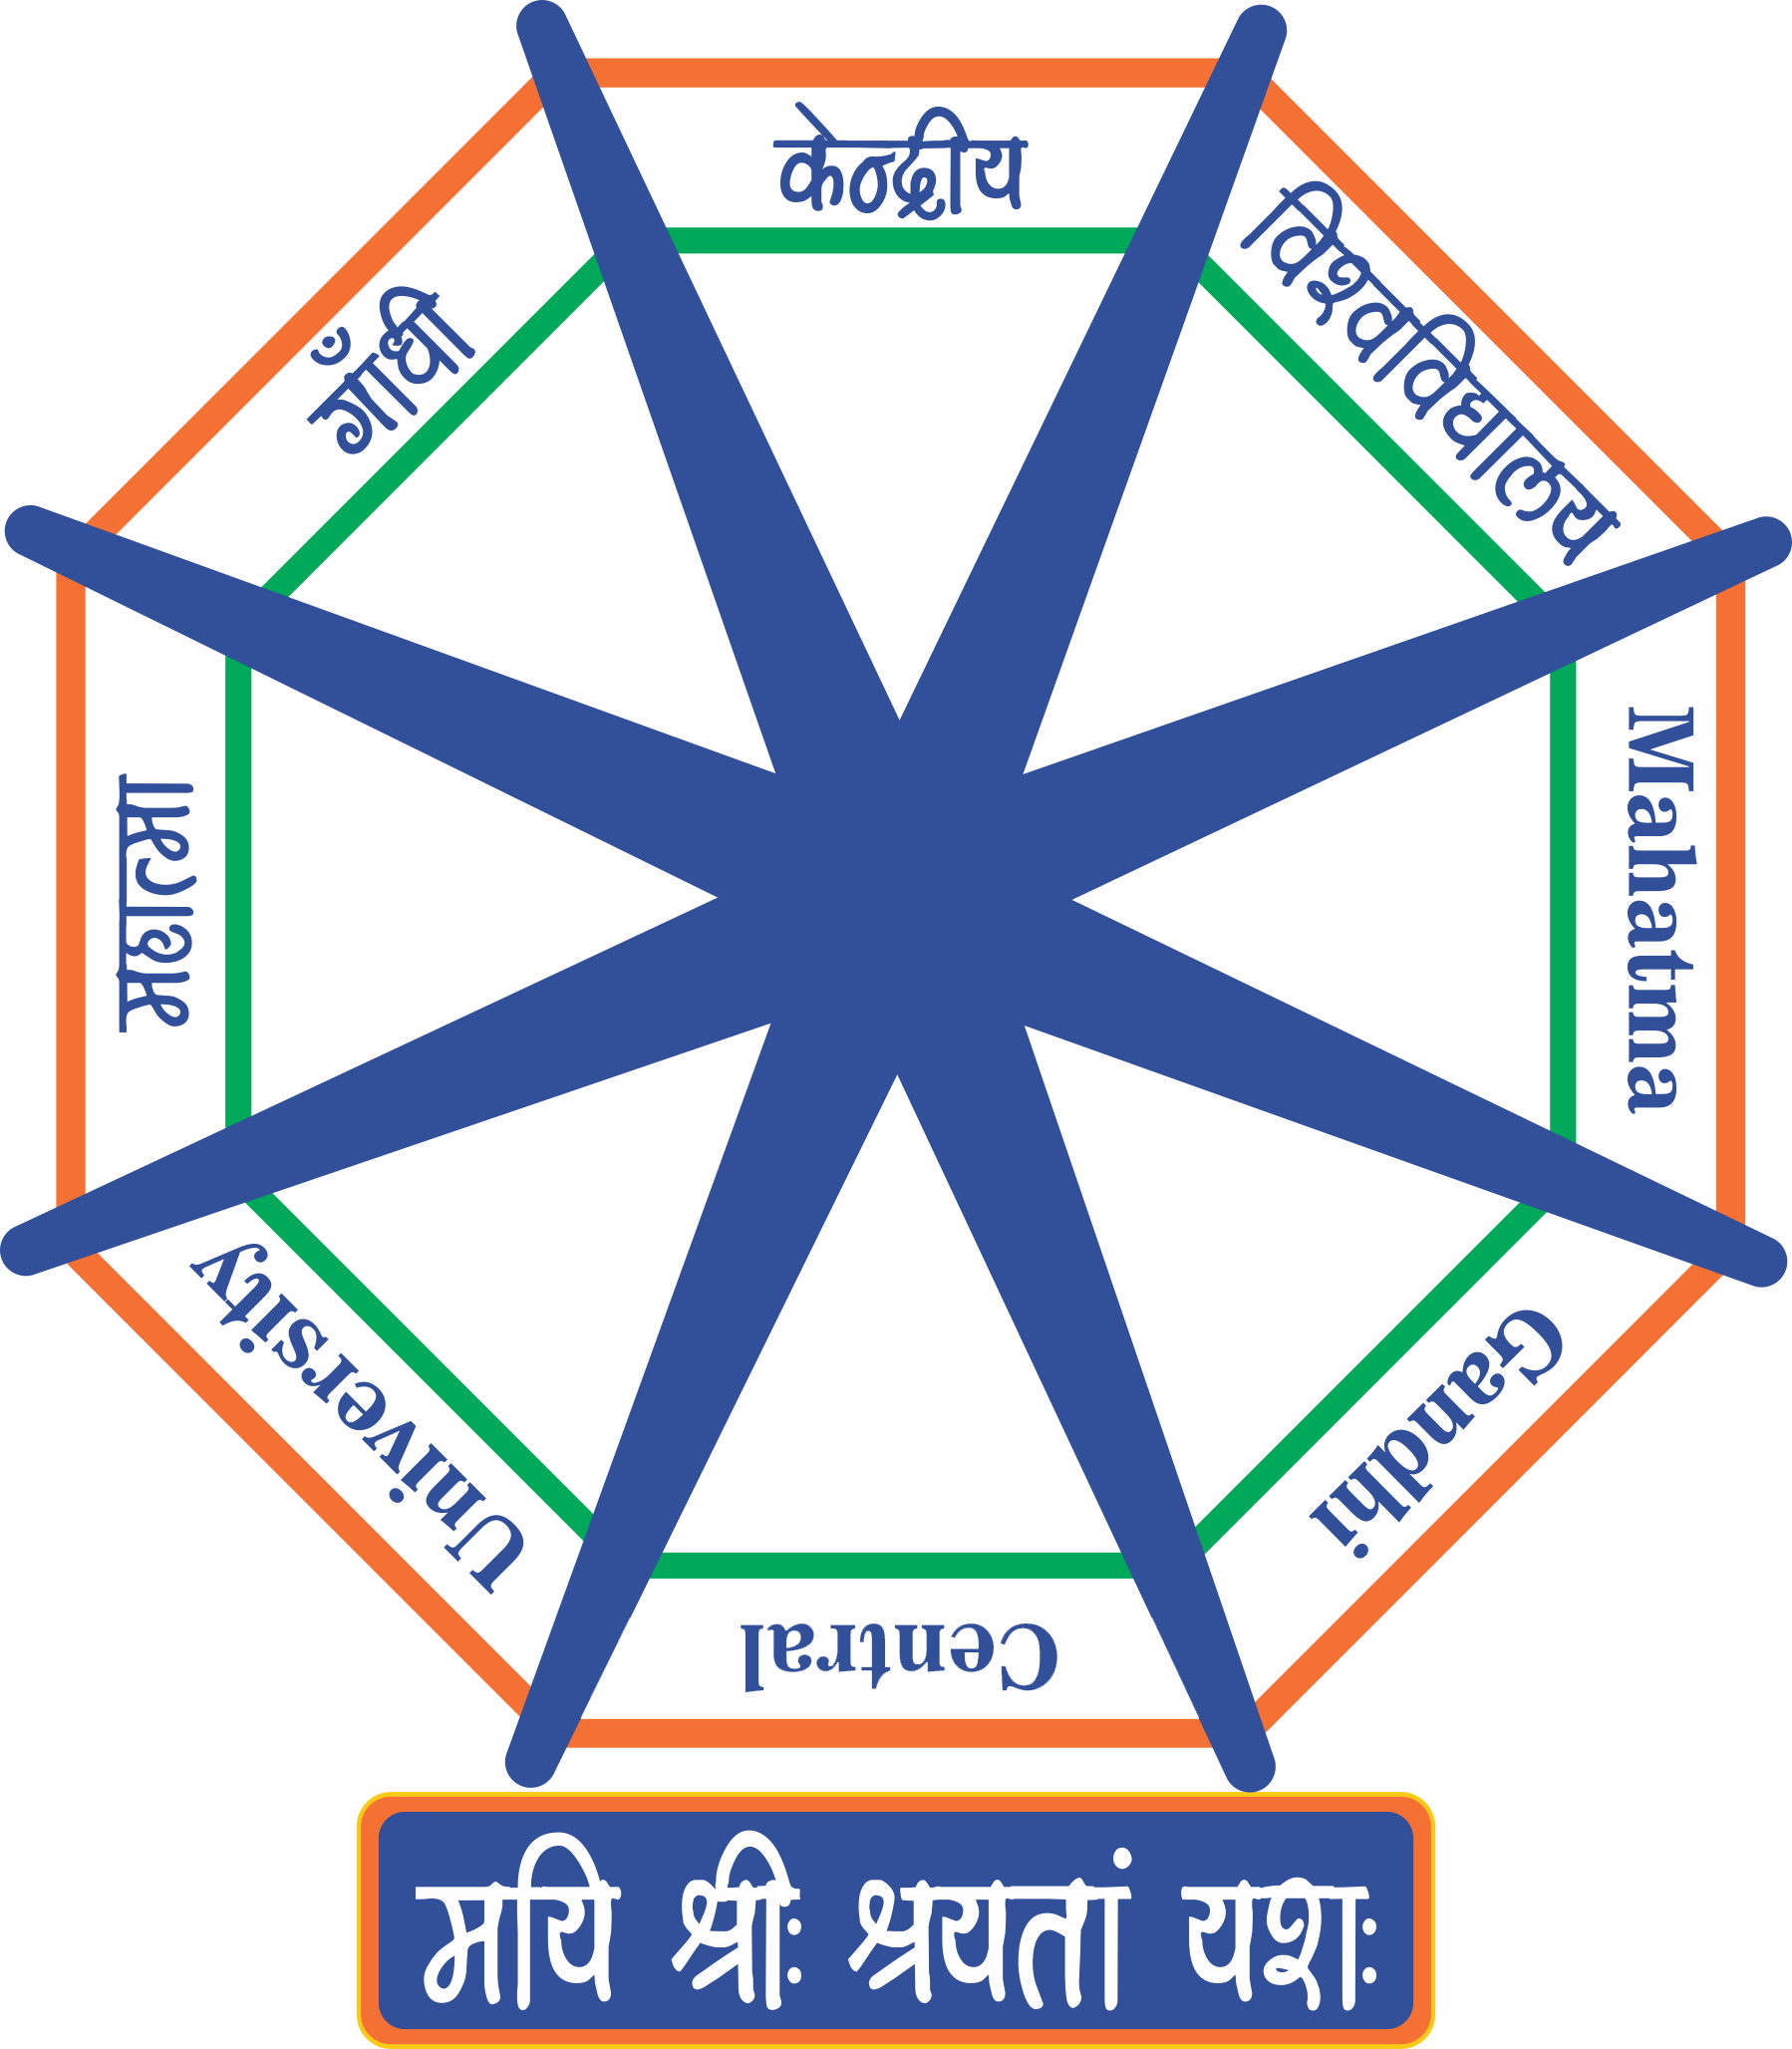
\includegraphics[width=1\textwidth]{mgcu}
    \caption{Actual vs Predicted of BiLSTM for All Datasets}
    \label{img:bilstn_a_p}
\end{figure}
